\chapter{Functional Derivatives}
\label{section:Functional derivative}
Functional derivatives generalize the notion of a gradient and the directional derivative.
A function $f(p)$, where $p$ is point with coordinates $x_i = x_i(p)$, has a gradient
\begin{equation}
    \dd f_p = \pdv{f(p)}{x_i} \dd x_i.
\end{equation}
The derivative in a particular direction $v = v^i \partial_i$ is 
\begin{equation}
    \dv{\epsilon} f(x_i + \epsilon v_i) = f(x) + \dd f_x (v) = f(x) + \pdv{f}{x^i}v_i.
\end{equation}
This is generalized to functionals through the definition of the functional derivative and the variation of a functional.
Let $F[f]$ be a functional, i.e., a machine that takes in a function and returns a number.
The obvious example in our case is the action, which takes in one or more field configurations, and returns a single real number.
We will assume here that the functions have the domain $\Omega$, with coordinates $x$.
The functional derivative is defined as
\begin{equation}
    \delta F[f]
    =
    \dv{\epsilon} F[f + \epsilon \eta] \Big|_{\epsilon = 0}
    = \int_\Omega \dd x \, \frac{\delta F[f]}{\delta f(x)} \eta(x).
\end{equation}
$\eta(x)$ is here an arbitrary function, but we will make the important assumption that it as well as all its derivatives are zero at the boundary of its domain $\Omega$.
This allows us to discard surface terms stemming from partial integration, which we will use frequently.
We may use the definition to derive one of the fundamental relations of functional derivation.
Take the functional $F[f] = f(x)$. 
Then,
\begin{equation}
    \label{Functional derivative delta identity}
    \delta F[f] = \dv{\epsilon} [f(x) + \epsilon \eta(x)] = \eta(x) = \int \dd y \, \delta(x - y) \eta(y)
\end{equation}
This leads to the identity
\begin{equation}
    \frac{\delta f(x)}{\delta f(y)} = \delta(x - y),
\end{equation}
for any function $f$.
Higher functional derivatives are defined similarly, by applying functional variation repeatedly
\begin{equation}
    \delta^n F[f] = \dv{\epsilon} \delta^{n-1}F[f + \epsilon \eta_n] \big|_{\epsilon=0}
    = \int \left(\prod_{i=1}^n \dd x_i\right)
    \frac{\delta^n F[f]}{ \delta f(x_n)\dots\delta f(x_n)} \left(\prod_{i=1}^n \eta_i(x_i)\right).
\end{equation}
A functional may be expanded in a generalization of the Fourier series, which has the form
\begin{equation}
    F[f_0 + f] = F[f_0] + \int_\Omega \dd x \, f(x) \frac{\delta F[f_0]}{\delta f(x)}\bigg|_{f = f_0}
    + \frac{1}{2!}\int_\Omega \dd x \dd y \, f(x) f(y) \frac{\delta^2 F [f_0]}{\delta f(x) \delta f(y)}
    + \dots
\end{equation}
As an example, the Klein-Gorodn action
\begin{equation}
    S[\varphi] = - \frac{1}{2}\int_\Omega \dd x \, \varphi (\partial^2 + m^2) \varphi(x)
\end{equation}
can be evaluated quickly by using \autoref{Functional derivative delta identity} and partial integration
\begin{align}
    \nonumber
    \funcdv{\varphi(x)} S[\varphi] 
    & = 
    - \frac{1}{2} \int_\Omega \dd y \, 
    [\delta(x - y)(\partial_y^2 + m^2)\varphi(y) + \varphi(y) (\partial_y^2 + m^2)\delta(x - y)] \\
    & = 
    - \int_\Omega \dd y \, 
    \delta(x - y)(\partial_y^2 + m^2)\varphi(y) 
    = (\partial_x^2 + m^2)\varphi(x)
\end{align}
The second derivative is
\begin{equation}
    \frac{\delta^2S[\varphi]}{\delta \varphi(x)\delta \varphi(y)}
    =
    \funcdv{\varphi(x)} (\partial_y^2 + m^2)\varphi(y)
    = 
    (\partial_y^2 + m^2) \delta(x - y).
\end{equation}


\subsection*{Gaussian integrals}
\label{section:gaussian integrals}

\begin{figure}[ht]
    \centering
    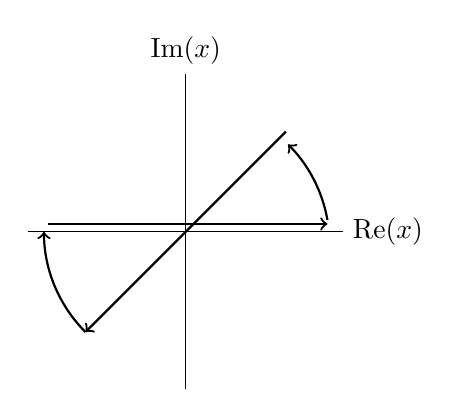
\begin{tikzpicture}
        \draw (-2, 0) -- (2, 0) node[right] {$\mathrm{Re}(x)$};
        \draw (0, -2) -- (0, 2) node[above] {$\mathrm{Im}(x)$};
        \draw[->, thick] (-1.75, 0.1) -- (1.8, 0.1);
        \draw[->, thick] (1.8, 0.15) arc (10:45:1.8);
        \draw[->, thick] ({1.8/sqrt(2)}, {1.8/sqrt(2)}) -- ({-1.8/sqrt(2)}, {-1.8/sqrt(2)});
        \draw[->, thick] ({-1.8/sqrt(2)}, {-1.8/sqrt(2)}) arc (225:180:1.8);
    \end{tikzpicture}
    \caption{Wick rotation}
    \label{Wick rotation}
\end{figure}


A useful integral is the Gaussian integral,
\begin{equation}
    \int_\R \dd z \, \exp(- \frac{1}{2} a z^2) = \sqrt{\frac{2 \pi}{a}},
\end{equation}
for $a \in \R$. The imaginary version,
\begin{equation}
    \int_R \dd z \, \exp(i \frac{1}{2} a z^2 )
\end{equation}
does not converge. However, if we change $a \rightarrow a + i\epsilon$, the integrand is exponentially suppressed.
\begin{equation}
    f(x) = \exp(i \frac{1}{2}a x^2) \rightarrow
    \exp(i\frac{1}{2}a x^2 - \frac{1}{2} \epsilon  x^2).
\end{equation}
As the integrand falls exponentially for $x\rightarrow \infty$ and contains no poles in the upper right nor lower left quarter of the complex plane, we may perform a wick rotation by closing the contour as shown in \autoref{Wick rotation}.
This gives the result
\begin{equation}
    \label{complex gauss 1D}
    \int_\R \dd x \, \exp(i \frac{1}{2}(a + i\epsilon) x^2) 
    = \int_{\sqrt{i}\R} \dd x \, \exp(i\frac{1}{2} ax^2)
    = \sqrt{i} \int_\R \dd y\, \exp(-\frac{1}{2} (-a) y^2) = \sqrt{\frac{2 \pi i}{(-a)}}
\end{equation}
where we have made the change of variable $y = (1+i)/\sqrt{2} x = \sqrt{i} x$.
In $n$ dimensions, the Gaussian integral formula generalizes to
\begin{equation}
    \int_{\R^n} \dd^n x \, \exp{-\frac{1}{2} x_n A_{nm} x_m } =\sqrt{\frac{(2 \pi)^n}{\det(A)}},
\end{equation}
where $A$ is a matrix with $n$ real, positive eigenvalues.
We may also generalize \autoref{complex gauss 1D},
\begin{align}
    \int_{\R^n} \dd^n x \, \exp{i\frac{1}{2} x_n( A_{nm} + i \epsilon \delta_{nm}) x_m } =\sqrt{\frac{(2 \pi i )^n}{\det(-A)}}.
\end{align}
The final generalization is to functional integrals,
\begin{align}
    \int \D \varphi \, \exp(- \frac{1}{2} \int \dd x \, \varphi(x) A \varphi(x) )
    = C (\det(A))^{-1/2},
    \int \D \varphi \, \exp(i\frac{1}{2} \int \dd x \, \varphi(x) A \varphi(x) )
    = C (\det(-A))^{-1/2}.
\end{align}
$C$ is here a divergent constant, but will either fall away as we are only looking at the logarithm of $I_\infty$ and are able to throw away additive constants, or ratios between quantities which are both multiplied by $C$.

The Gaussian integral can be used for the stationary phase approximation.
In one dimension, it is
\begin{equation}
    \int \dd x \, \exp(i \alpha f(x)) 
    \approx \sqrt{\frac{2 \pi }{f''(x_0)}}\exp( f(x_0)), 
    \, f'(x) = 0, \, \alpha\rightarrow \infty
\end{equation}
The functional generalization of this is
\begin{equation}
    \int \D \varphi \exp{i S[\varphi]}
    \approx 
    C \det(- \frac{\delta^2 S[\varphi_0]}{\delta \varphi^2})
    \exp{i \alpha S[\varphi_0]  }, \quad
    \frac{\delta S[\varphi_0]}{\delta \varphi} = 0…
\end{equation}
Here, $S[\varphi]$ is a general functional of $\varphi$, and we have used the Taylor expansion, and $\varphi_0$ fulfills
\begin{equation}
    \funcdv{\varphi(x)}{S[\varphi_0]} = 0,
\end{equation}

